%-----------------------------------------------------------------------------%
%                                                                             %
%    K A P I T E L   1                                                        %
%                                                                             %
%-----------------------------------------------------------------------------%

\chapter{Introduction}\label{c1}
\section{Motivation}
\section{Related Work}
%\subsection{Model Induced Design} (Passive Dynamic Walking, Template Models)
%\subsection{Traditional Legged Locomotion Planning}
%\subsection{Trajectory Optimization} (Sequential, Simultaneous OR Direct, Indirect, DDP)
%\subsection{Series-Parallel Hybrid Robots}
\section{Contribution}
\section{Structure}


\section{RH5 Humanoid Robot}
The derived approaches for constrained \gls{DDP} have been tested both in simulation and real-world experiments on a full-size humanoid robot. RH5 is a lightweight and biologically inspired humanoid robot that has recently been developed at DFKI Robotics Innovation Center.  \cite{peters2017konstruktion}.

The robot contains   

\begin{figure}[h!]
\centering	
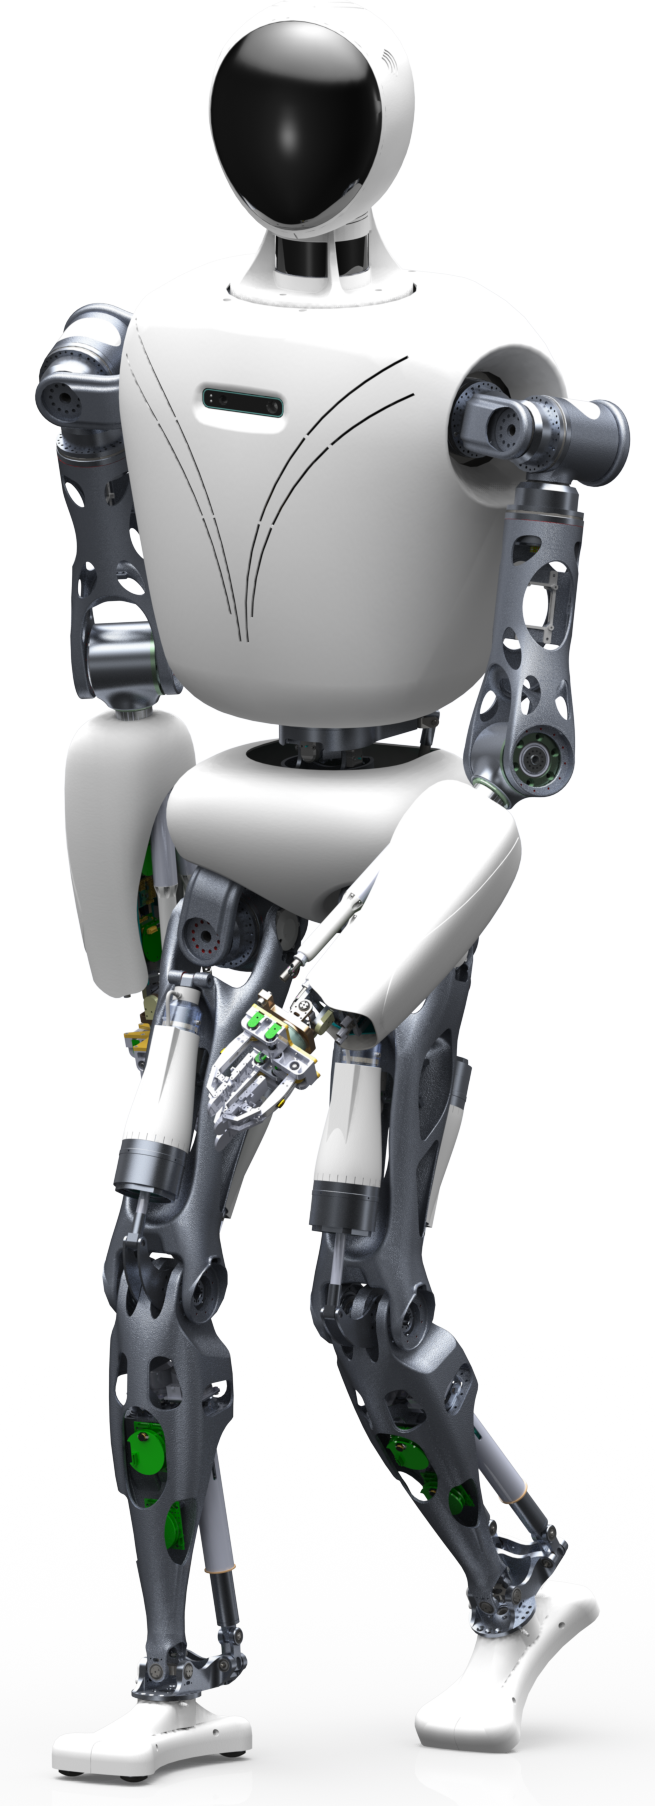
\includegraphics[width=.25\textwidth]{img/rh5_robot.png}
\caption{The recently presented RH5 humanoid containing series-parallel mechanisms.}
\label{fig:rh5}
\end{figure} 


